\chapter{Deep Latent Variables Generative Models}\label{ch:03}

\begin{chapter_outline}

  In this chapter, we demonstrate that combining distinct class of models is benefitial. In particular, we study the complementary of variational autoencoders (VAEs) and denoising diffusion probabilistic models (DDPMs). VAEs offer scalable amortized posterior inference and fast sampling but are also more and more outperformed by competing models such as normalizing flows (NFs) or deep-energy models. We improve VAEs by modelling the prior distribution of the latent variables with a diffusion process. The diffusion prior model improves upon Gaussian priors of classical VAEs and is competitive with NF-based priors.
  This contribution shows that connecting different classes of deep probabilistic models can unlock new modelling capacity and properties that are unreachable by each class of models independently.
\end{chapter_outline}
\section{Prologue}
The role of this chapter is to demonstrate, with a simple example, that different (deep) probabilistic models shall not be studied independently. Instead, building a broad understanding of all these models allows us to try an almost infinite set of combinations, each owning distinct properties. Each class of models has its own assets and limitations but combining two models together can help in reducing the weaknesses of the two classes of models while maintaining their benefits.

The unified training framework of neural networks unlocks the creation of ``super'' deep probabilistic models that combines together many types of probabilistic models. Indeed, it is nowadays very natural to parameterize probabilistic models with neural networks. In these cases, models share a unique training procedure based on stochastic gradient descent. This allows the joint optimization of all components of a `super` model composed of distinct types of DPMs as long as we can express the final objective as a function of these models.

As will see later in this paper, combining DDPMs and VAEs is fairly straighforward and it easily leads to better modelling for image synthesis. We believe that fostering further the interplay between different DPMs is important in the development of probabilistic modelling toolbox. In particular, these tools should naturally be part of the building blocks of any probabilistic programming language and combining them should be as simple as replacing a Normal distribution by a Laplace distribution in a probabilistic program.

\section{The paper: Diffusion Priors In Variational Autoencoders}

\subsection{Author contributions}
The paper is co-authored by me and Gilles Louppe. As the leading author, I developed the connections between diffusion models and variational autoencoders, made the experiments, and wrote the paper. In particular, I derived the ELBO associated to the denoising diffusion priors in VAES. Gilles Louppe supervised me throughout this project, offered suggestions and helped in writing the paper.

\subsection{Reading tips}
The reader may skip section 2 which presents VAEs and DDPMs already introduced the background chapter. The reader interested in deeply understanding the implementation of DDPMs should take a look at \citet{ho_denoising_2020}. The rest of the paper should flow naturally.

% \subsection{Minor corrections}

\includepdf[pages=-]{papers/innf_latent_diffusion.pdf}

\section{Epilogue}
\subsection{Scientific impact}

According to Google Scholar, our article has received five citations between its publication in June 2021 and July 2022. We shall contrast this number with the 48 citations received by \citet{vahdat2021score}, which was published in December 2021 at NeurIPS 2021 and was first released as a preprint on Arxiv in June 2021. Although the ideas expressed in the two papers are similar, our work did not gain as much visibility as theirs. We acknowledge at least three fair reasons to explain this. First, publishing at NeurIPS brings much more visibility than at a workshop at ICML. This is natural as the reviewing process of NeurIPS is much stronger. Second, \citet{vahdat2021score} achieve state-of-the-art image synthesis by combining their idea with the proper neural architectures, training tricks and computation power.
In contrast, our work is a proof of concept and does not achieve state-of-the-art performance. In this regard, our work is preliminary compared to theirs. Finally, advertising science is arguably nowadays as important as the science itself in machine learning.\citet{vahdat2021score} made an excellent job, as can be seen by one tweet from the first author who advertised their paper in \Cref{fig:cont_tweet} and had $6\times$ higher reach than a similar advertisement by Gilles Louppe in \Cref{fig:discrete_tweet}.

Since the publication of this article, diffusion models have become very popular, owing their success to the astonishing results achieved by large text-to-images models created by OpenAI~\citep[$\text{DALL}\cdot\text{E} 2$][]{ramesh2022hierarchical} and Google~\citep[Imagen][]{saharia2022photorealistic}. Close to our work, \citet{yu2022latent} recently proposed to use energy based models trained with denoising score matching to model the prior distribution of VAEs for interpretable text modelling.

Our initial motivation for combining diffusion models and VAEs was for enabling other type of noise for training diffusion models. Intuitively, the noise model provides an inductive bias to the learning algorithm, and adapting the noise to the data modality might help learning a better generative model. In particular, we thought heat equations would provide an appealing inductive bias for image synthesis as this equation tends to blur image along which corresponds to first destroying details from the image first and the semantic content toward the end. Our idea was to use the VAE formulation to bypass the closed form kernel required for obtaining a tractable training objective. In addition, we thought playing with different diffusion speed inside the latent variables of the VAE would eventually enforce different levels of structure between latent variables with different diffusion schedules. This would have provided an elegant way of extracting high and low level semantic from images and to create interesting applications based on conditional generative modelling. Unfortunately, I did not figure out how making these models work appropriately to start writing a publication. It is interesting to observe that recently, \citet{rissanen2022generative} had a similar idea and managed to achieve state-of-the-art image synthesis with a diffusion model based on the heat equation instead of the diffusion equation. In the future, it would be worth seeing if such inductive bias can be helped by VAEs like latent models to compress data into human-interpretable features.


\begin{figure*}
  \centering
  \begin{subfigure}[b]{.48\textwidth}
    \centering
    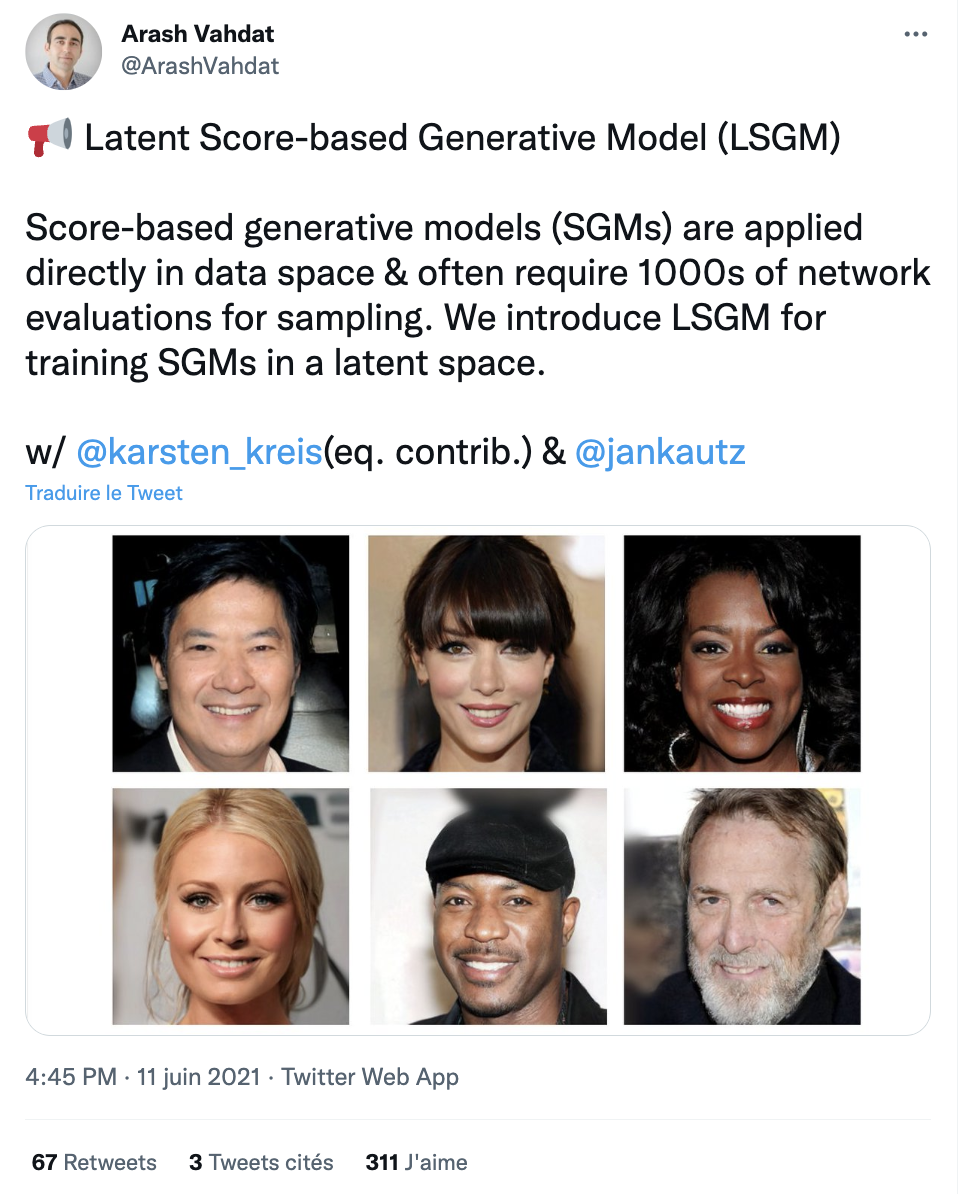
\includegraphics[width=.95\textwidth]{figures/impact_scholar/cont_diff_tweet.png}
    \caption{}
    \label{fig:cont_tweet}
  \end{subfigure}
  \begin{subfigure}[b]{.48\textwidth}
    \centering
    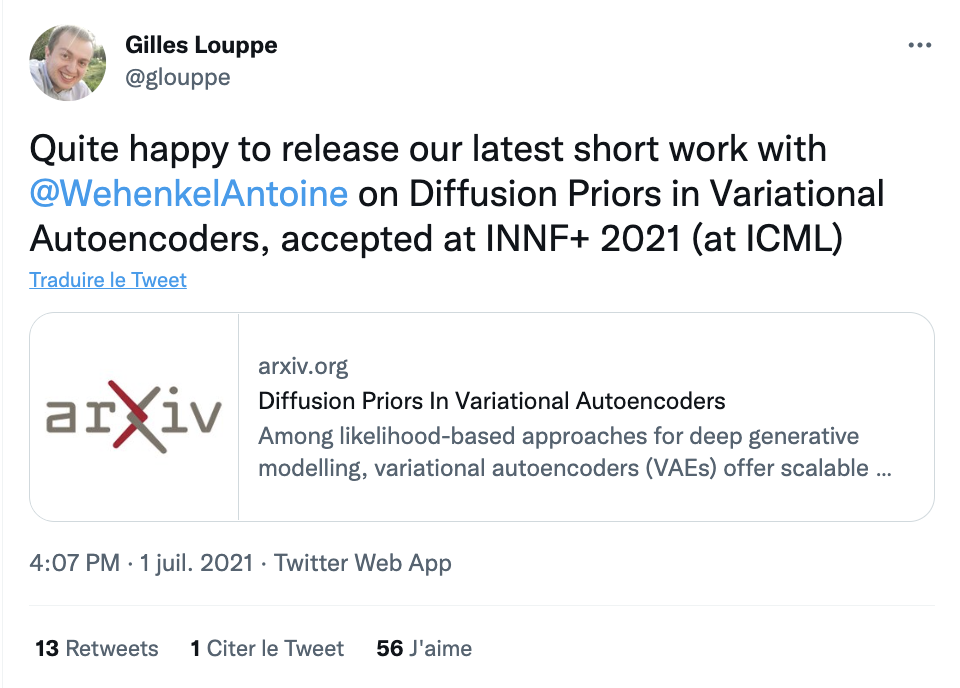
\includegraphics[width=.95\textwidth]{figures/impact_scholar/discret_diff_tweet.png}
    \caption{}
    \label{fig:discrete_tweet}
  \end{subfigure}
  \caption{Tweets advertising (\textbf{a}) The continuous-time diffusion models in the latent space from \citet{vahdat2021score} (\textbf{b}) The discrete-time diffusion models in the latent space from ours.}
\end{figure*}
